\documentclass[fleqn]{article}

%% Created with wxMaxima 25.01.0

\setlength{\parskip}{\medskipamount}
\setlength{\parindent}{0pt}
\usepackage{iftex}
\ifPDFTeX
  % PDFLaTeX or LaTeX 
  \usepackage[utf8]{inputenc}
  \usepackage[T1]{fontenc}
  \DeclareUnicodeCharacter{00B5}{\ensuremath{\mu}}
\else
  %  XeLaTeX or LuaLaTeX
  \usepackage{fontspec}
\fi
\usepackage{graphicx}
\usepackage{color}
\usepackage[leqno]{amsmath}
\usepackage{ifthen}
\newsavebox{\picturebox}
\newlength{\pictureboxwidth}
\newlength{\pictureboxheight}
\newcommand{\includeimage}[1]{
    \savebox{\picturebox}{\includegraphics{#1}}
    \settoheight{\pictureboxheight}{\usebox{\picturebox}}
    \settowidth{\pictureboxwidth}{\usebox{\picturebox}}
    \ifthenelse{\lengthtest{\pictureboxwidth > .95\linewidth}}
    {
        \includegraphics[width=.95\linewidth,height=.80\textheight,keepaspectratio]{#1}
    }
    {
        \ifthenelse{\lengthtest{\pictureboxheight>.80\textheight}}
        {
            \includegraphics[width=.95\linewidth,height=.80\textheight,keepaspectratio]{#1}
            
        }
        {
            \includegraphics{#1}
        }
    }
}
\newlength{\thislabelwidth}
\DeclareMathOperator{\abs}{abs}

\definecolor{labelcolor}{RGB}{100,0,0}

\begin{document}
Given the function


\noindent
%%%%%%%%
%% INPUT:
\begin{minipage}[t]{4.000000em}\color{red}\bfseries
(\% i1)	
\end{minipage}
\begin{minipage}[t]{\textwidth}\color{blue}
f(x):=(3*x+15*x\^\ 2-x\^\ 4)/(9*x\^\ 2+1);
\end{minipage}
%%%% OUTPUT:
\[\displaystyle \tag{\% o1} 
\mathop{f}(x)\mathop{:=}\frac{3 x\mathop{+}15 {{x}^{2}}\mathop{-}{{x}^{4}}}{9 {{x}^{2}}\mathop{+}1}\mbox{}
\]
%%%%%%%%%%%%%%%%
(a) The graph of f(x) is


\noindent
%%%%%%%%
%% INPUT:
\begin{minipage}[t]{4.000000em}\color{red}\bfseries
(\% i2)	
\end{minipage}
\begin{minipage}[t]{\textwidth}\color{blue}
wxplot2d(f(x),\ [x,\ -5,\ 5],\ [y,\ -1,\ 2]);
\end{minipage}
%%%% OUTPUT:
\[\displaystyle plot2d: some values will be clipped.
\mbox{}\]

\[\tag{\% t2} 
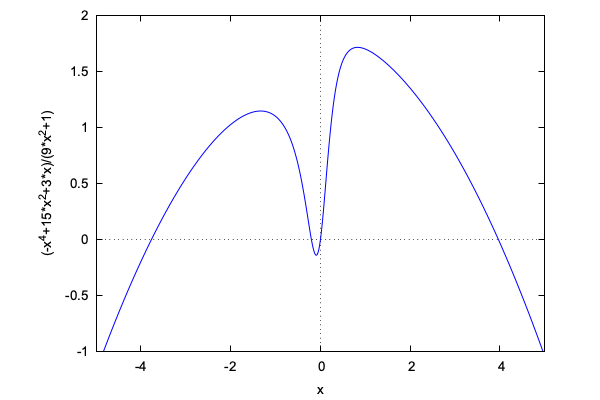
\includegraphics[width=.95\linewidth,height=.80\textheight,keepaspectratio]{question_7_img/question_7_1}\mbox{}\]

\[\tag{\% o2} 
\mbox{}
\]
%%%%%%%%%%%%%%%%
(b) the derivative of f(x) is


\noindent
%%%%%%%%
%% INPUT:
\begin{minipage}[t]{4.000000em}\color{red}\bfseries
(\% i3)	
\end{minipage}
\begin{minipage}[t]{\textwidth}\color{blue}
df(x):=''(diff(f(x),\ x));
\end{minipage}
%%%% OUTPUT:
\[\displaystyle \tag{\% o3} 
\mathop{df}(x)\mathop{:=}\frac{\mathop{-}\left( 4 {{x}^{3}}\right) \mathop{+}30 x\mathop{+}3}{9 {{x}^{2}}\mathop{+}1}\mathop{-}\frac{18 x\, \left( \mathop{-}{{x}^{4}}\mathop{+}15 {{x}^{2}}\mathop{+}3 x\right) }{{{\left( 9 {{x}^{2}}\mathop{+}1\right) }^{2}}}\mbox{}
\]
%%%%%%%%%%%%%%%%
(c)  The positive local maximum of f(x) is


\noindent
%%%%%%%%
%% INPUT:
\begin{minipage}[t]{4.000000em}\color{red}\bfseries
(\% i4)	
\end{minipage}
\begin{minipage}[t]{\textwidth}\color{blue}
pos\_root:find\_root(df(x),\ x,\ 0,\ 5);
\end{minipage}
%%%% OUTPUT:
\[\displaystyle \tag{pos\_ root} 
0.8288158368533624\mbox{}
\]
%%%%%%%%%%%%%%%%
Substituting this back into the f(x)


\noindent
%%%%%%%%
%% INPUT:
\begin{minipage}[t]{4.000000em}\color{red}\bfseries
(\% i5)	
\end{minipage}
\begin{minipage}[t]{\textwidth}\color{blue}
f(pos\_root);
\end{minipage}
%%%% OUTPUT:
\[\displaystyle \tag{\% o5} 
1.71510439942526\mbox{}
\]
%%%%%%%%%%%%%%%%
Finding the second derivative of f(x)


\noindent
%%%%%%%%
%% INPUT:
\begin{minipage}[t]{4.000000em}\color{red}\bfseries
(\% i6)	
\end{minipage}
\begin{minipage}[t]{\textwidth}\color{blue}
ddf(x):=''(diff(df(x),\ x));
\end{minipage}
%%%% OUTPUT:
\[\displaystyle \tag{\% o6} 
\mathop{ddf}(x)\mathop{:=}\frac{30\mathop{-}12 {{x}^{2}}}{9 {{x}^{2}}\mathop{+}1}\mathop{-}\frac{18 \left( \mathop{-}{{x}^{4}}\mathop{+}15 {{x}^{2}}\mathop{+}3 x\right) }{{{\left( 9 {{x}^{2}}\mathop{+}1\right) }^{2}}}\mathop{+}\frac{648 {{x}^{2}} \left( \mathop{-}{{x}^{4}}\mathop{+}15 {{x}^{2}}\mathop{+}3 x\right) }{{{\left( 9 {{x}^{2}}\mathop{+}1\right) }^{3}}}\mathop{-
}\frac{36 x\, \left( \mathop{-}\left( 4 {{x}^{3}}\right) \mathop{+}30 x\mathop{+}3\right) }{{{\left( 9 {{x}^{2}}\mathop{+}1\right) }^{2}}}\mbox{}
\]
%%%%%%%%%%%%%%%%
And substitutiong our x variable


\noindent
%%%%%%%%
%% INPUT:
\begin{minipage}[t]{4.000000em}\color{red}\bfseries
(\% i7)	
\end{minipage}
\begin{minipage}[t]{\textwidth}\color{blue}
ddf(0.829);
\end{minipage}
%%%% OUTPUT:
\[\displaystyle \tag{\% o7} 
\mathop{-}1.2681397331452517\mbox{}
\]
%%%%%%%%%%%%%%%%
As this is \ensuremath{<}0 the point is confirmed to be a local maximum of f(x)
Hence the local maximum is at (0.828,1.715), to 3 d.p.
(d) To find the root to the right of x=0


\noindent
%%%%%%%%
%% INPUT:
\begin{minipage}[t]{4.000000em}\color{red}\bfseries
(\% i8)	
\end{minipage}
\begin{minipage}[t]{\textwidth}\color{blue}
float(realroots(f(x)));
\end{minipage}
%%%% OUTPUT:
\[\displaystyle \tag{\% o8} 
\mathop{[}x\mathop{=}\mathop{-}3.7688187062740326\mathop{,}x\mathop{=}\mathop{-}0.20053765177726746\mathop{,}x\mathop{=}3.9693563878536224\mathop{,}x\mathop{=
}0.0\mathop{]}\mbox{}
\]
%%%%%%%%%%%%%%%%
Therefore the grapg crosses the x-axis at 3.969, to 3 d.p.
The area under the graph between x=0 and this point is


\noindent
%%%%%%%%
%% INPUT:
\begin{minipage}[t]{4.000000em}\color{red}\bfseries
(\% i10)	
\end{minipage}
\begin{minipage}[t]{\textwidth}\color{blue}
quad\_qags(f(x),\ x,\ 0,\ 3.969);
\end{minipage}
%%%% OUTPUT:
\[\displaystyle \tag{\% o10} 
\left[ 4.342959640603124\mathop{,}2.5621777856375642 {{10}^{-9}}\mathop{,}105\mathop{,}0\right] \mbox{}
\]
%%%%%%%%%%%%%%%%
Hence the area enclosed by the graph of f(x) between 0\ensuremath{<}=x\ensuremath{<}=3.969 is 4.343, to 3 d.p.
\end{document}
